\documentclass[letterpaper]{article}
\usepackage{aaai}
\usepackage{aaai}
\usepackage{times}
\usepackage{helvet}
\usepackage{courier}
\usepackage{graphicx}
\usepackage{algorithm}
\usepackage{algpseudocode}
\usepackage{amsmath}

% comment out this line to disable inline comments
\def\draft{}
\linespread{0.99}

\usepackage{color}
\usepackage{amsmath, amsfonts, amssymb}

\usepackage{subfig}

\def\rx{{\texttt{T-REX\ }}}
\def\rxe{{\texttt{T-REX}}}
\def\eut{{\texttt{EUROPA}$_2$\ }}
\def\eu{{\texttt{EUROPA}\ }}
\def\eue{{\texttt{EUROPA}}}
\def\eus{{\texttt{EUROPA}'s\ }}
\def\nd{{\texttt{NDDL\ }}}
\def\nde{{\texttt{NDDL}}}
\def\mb{{\texttt{MBFD\ }}}
\def\mbe{{\texttt{MBFD}}}
\def\WW{{\texttt{WireWalker\ }}}
\def\WWe{{\texttt{WireWalker}}}

\def\etal{{et al.\/}}
\def\eg{e.g., }
\def\ie{{i.e.,\ }}
\def\etc{{etc.\ }}
\def\situ{{in situ \/}}
\def\PN{{\emph{PN} }}
\def\can{{\texttt{CANON\ }}}
\def\od{{\texttt{ODSS\ }}}
\def\ode{{\texttt{ODSS}}}

\newtheorem{Prop}{Proposition}
\newtheorem{Theorem}{Theorem}
\newtheorem{Lemma}{Lemma}
\newtheorem{Corrolary}{Corollary}
\newtheorem{definition}{Definition}

%\setlength{\marginparwidth}{8mm}

\usepackage{xcolor}

\ifdefined\draft 
  \usepackage{pdfcomment}

  \newcommand{\comment}[2]{\pdfcomment[#1]{#2}}
  \newcommand{\highlight}[2]{\pdfmarkupcomment[#1]{#2}{}}
\else
  \newcommand{\comment}[2]{}
  \newcommand{\highlight}[2]{#2}
\fi

\newcommand{\kcomment}[1]{\comment{author=Kanna,color=red}{KR: #1}}
\newcommand{\fcomment}[1]{\comment{author=Frederic,color=gray}{FP: #1}}
\newcommand{\pcomment}[1]{\comment{author=Philip,color=yellow}{PC: #1}}


\newcommand{\khighlight}[1]{\highlight{author=Kanna,color=red}{#1}}
\newcommand{\fhighlight}[1]{\highlight{author=Frederic,color=gray}{#1}}
\newcommand{\phighlight}[1]{\comment{author=Philip,color=yellow}{#1}}



\begin{document}
\title{Anticipatory Continuous Robotic Plan Execution}
\author{Paper \# 88}
% \author{Philip Cooksey \And Fr\'ed\'eric Py \And Paul Morris \And Kanna Rajan}
\maketitle{}

\begin{abstract}

  Robotic plan execution has traditionally assumed that goals are
  articulated prior to mission execution. As robots have become
  persistent and moved into the real-world, the need to anticipate and
  capture evolving needs with new or reformulated goals becomes
  critical.  We explore this issue not yet described in the literature.
  We then demonstrate a simple yet elegant initial approach to this
  problem motivated by our oceanographic domain.  A policy handler
  is sufficient to disambiguate actions for dispatch
  within a flexible temporal continuous plan execution system embedded
  within a robotic explorer.  The resulting algorithmic complexity is
  linear in the number of actions and causal links of an existing
  partial plan.

\end{abstract}

\section{Introduction}
\label{sec:intro}

As autonomous robots become more robust and persistent the likelihood
of their receiving new or modified objectives for tasking, during an
ongoing mission is high. Generative planning integrated within the
robotic architecture to fulfill current or such evolving agent
objectives and to deal with unanticipated situations is one approach
to enhance persistence while dealing with robot adaptation.  Earlier
work such as \texttt{IPEM} \cite{AmbrosIngerson88}, \texttt{ROGUE}
\cite{Haigh98}, and the LAAS architecture \cite{alami:1998p820} have
all contributed to this field of research. Results from such work have
lead to goal directed architectures that have sucessfully worked in
the real-world such as the Remote Agent Experiment \cite{mus98}, the
Autonomous Spacecraft Experiment \cite{chien99} and more recently the
Teleo Reactive Executive \cite{py10}. Often these architectures embed
planning engines that support a rich representation dealing with
durative actions and resources while ensuring partial plans are
flexible for robust execution \cite{lemai04}.  A resulting consequence
has been results in efficient approaches to temporal plan dispatch to
ensure robust and sound execution \cite{mus98a,morris01}. 

While these approaches have been necessary to correctly execute a
\emph{flexible temporal plan}, they view the agent itself as
synchronously fulfilling goals provided a priori, without the
introduction of new goals which could alter mission state and
execution.
% This oversight is understandable as such goals are by nature unknown
% and therefore impossible to integrate within the plan limiting the
% ability to formally take them into account.
The natural choice was to make the agent execute its actions as early
as the temporal plan and the current context would allow, with the
assumption that, the robot would finish its plan as early as possible
providing more 'temporal' room for potential future objectives.  This
can be problematic when new objectives are added during the course of
mission execution and especially pronounced with persistent
robots. For instance, the agent may prematurely task the robot to
leave an area of exploration (and exploitation) before an oncoming new
objective for this same geographical area is received resulting in
superfluous actions from the robot. Conversely, the robot waiting
inordinately could waste time with consequent lack of flexibility for
coping with diverse execution scenarios. In this context, it is
important for the agent to make a distinction between actions that can
be taken proactively versus other actions that may not be urgent.

In this work, we propose a systematic approach to allow the agent to
make such a distinction for each action by tracking causal
relationships between goals within the current plan. This allow us to
determine an appropriate dispatch strategy for execution, based on the
nature of the goals this action contributes to. While our approach
manipulates the plan structure, it is worth mentioning that it is
focused on more on plan execution within the agent than in the process
plan synthesis.  For the purposes of this paper, it allows us to
consider planning in abstraction while providing an anticipatory
approach to continuous robotic plan execution.

The structure of this paper is as follows. We motivate with an
scenario illustrating the problem of flexible plan execution, discuss
previous efforts with robotic controllers for planning and dispatching
for execution. We then present the algorithmic detail to solutions
that allow decision at execution time when planned actions should be
started. Finally, after presenting experimental results, we conclude
and discuss potential directions for future research.

%%% Local Variables: 
%%% mode: latex
%%% TeX-master: "aaai13"
%%% End: 


\paragraph{An Illustrative Example} 

Our focus of research is the oceanographic domain with a robotic
autonomous underwater vehicle (AUV) and illustrate issues arising with
dynamic goal emergence and motivate our approach.  In this domain an
AUV can either transit from one location to another within the water
mass or survey a location in order to collect data of a feature of
interest such as a hydrothermal vent depicted in
Fig. \ref{fig:Example}.  Note that the AUV must pass through {\em
  Vent1} to get to {\em Vent2}.  The vehicle is deployed initially
with the scientific objective to sample {\em Vent 2} and the
operational goal to be back at the {\em Surface} by the end of the
mission which lasts $12$ hours limited by its energy carrying
capacity. The support ship can send short commands and receive limited
data via limited acoustic communications.

%%%%%%%%%%%%%%%%%%
% Use the following if really needed
% \subfloat[\small Bathymetry of vent sites off of NW United States]{\label{fig:ex:axial}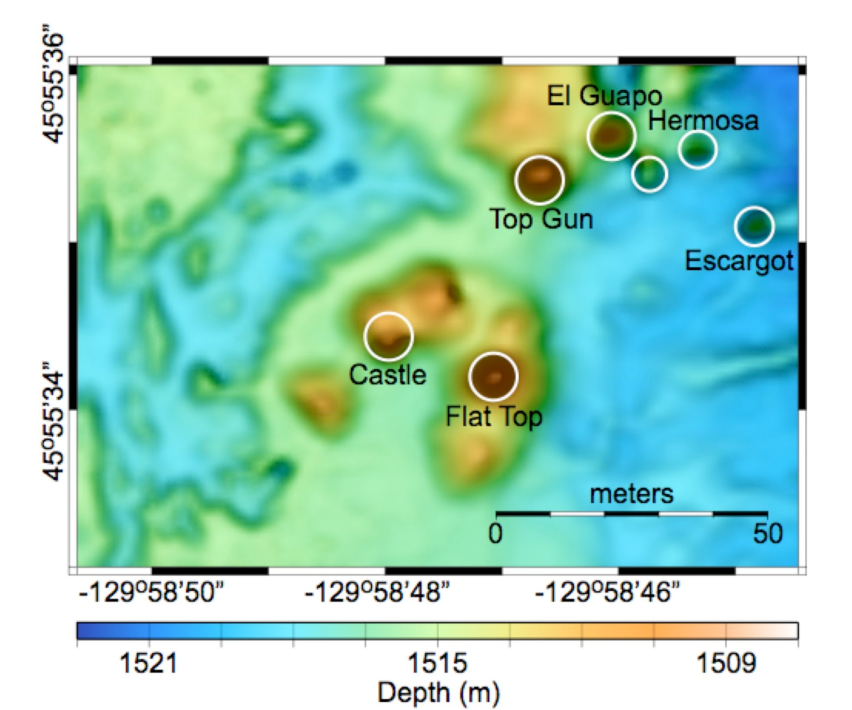
\includegraphics[scale=0.35]{figs/vents.pdf}}
%%%%%%%%%%%%%%%%%%
\begin{figure}[!t]
  \centering
  \subfloat[\small An illustration of our domain]{\label{fig:ex:graph}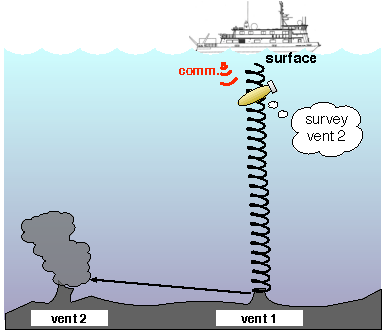
\includegraphics[width=0.51\columnwidth]{figs/auv_example}}
  \hfill \subfloat[\small Initial planning problem.]{\label{fig:ex:init}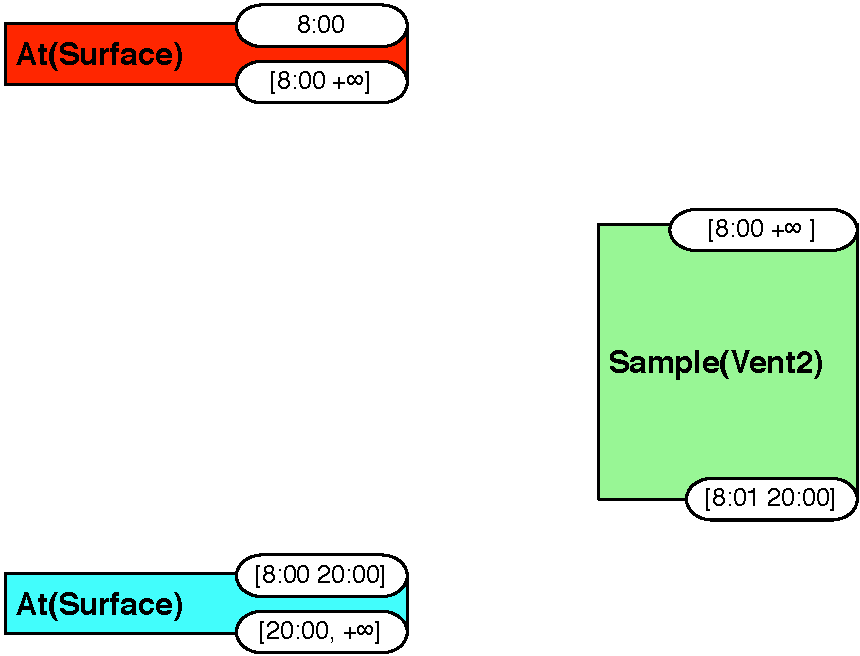
\includegraphics[width=0.49\columnwidth]{figs/example_initial}}
  \caption{\small{(\ref{fig:ex:graph}) illustrates the domain along
      with the initial partial plan for this problem
      (\ref{fig:ex:init}). The AUV is initially at {\em Surface} at
      8:00 and the mission is expected to complete by 20:00 with the
      goal --- marked with thick borders --- to sample {\em Vent 2}
      and the operational goal to be back at the surface for recovery
      by mission end.}}
  \label{fig:Example}
  \vskip-2mm
\end{figure}

The onboard planner produces the flexible temporal plan shown in
Fig. \ref{fig:ex:plan} for execution from the initial problem in
Fig. \ref{fig:ex:init}. However, at any time during the mission
scientists can decide, for example, that they also want to {\em
  sample} {\em Vent 1} as a consequence of data processing during the
traverse from the surface to {\em Vent 2}.  Time on site for such
bathymetric exploration is limited and expensive, so dynamic goal
generation is a reality.  Balancing between dispatching a plan action
\emph{proactive}ly or waiting till the latest start time is the
dichotomy the plan executive needs to resolve with consequent mission
efficiency impact.

% This raises the issue of balancing the decisions during plan execution
% between staring one plan action as early as possible --- which we will
% call {\em proactive} -- or wait until the action should necessarily
% start -- called later. There is a clear difference between the two
% approaches but when should, for example, the AUV wait or start early
% and how either will impact the mission execution when the new
% objective will be integrated by the AUV ?

\begin{figure}[!htb]
  \centering
  % \fcomment{In all the figures goals' color are the same "grey" as the
  %   other actions .... need to correct this.}
  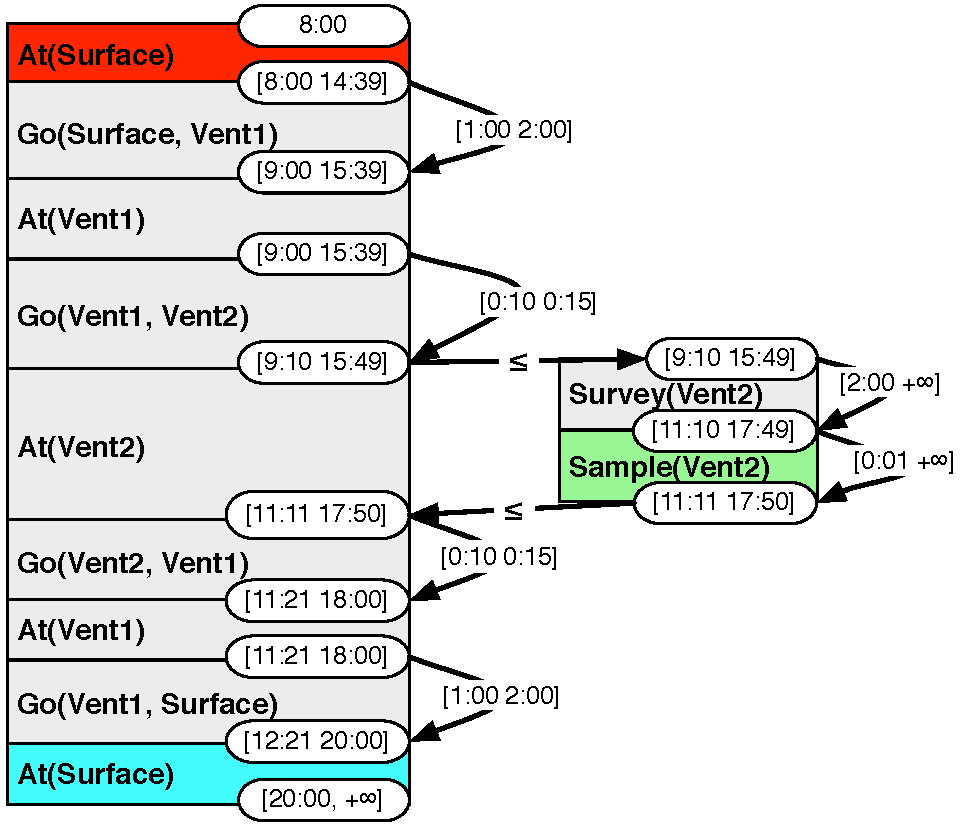
\includegraphics[width=0.8\columnwidth]{figs/example_plan}
  \vskip-2mm
  \caption{\small The flexible plan solution of the AUV domain in
    Fig. \ref{fig:Example}}
  \label{fig:ex:plan}
\end{figure}

Exclusively {\em deferring} the actions is not acceptable since it
results in the vehicle sitting at the surface, diving only at the very
last minute. If a new goal arrives subsequently, there is no time left
to do both objectives leaving the robot to exclude one of the goals or
fail to be at the surface as planned by 20:00. Equally, the {\em
  proactive} approach is problematic, since the vehicle will go
through the actions of the plan and be back at the surface early
(12:21). Even if the goal is provided early enough (by 14:00) the
vehicle will then have to dive back in order to survey and sample {\em
  Vent 1}.
% Even though the plan did initial provide a solution optimal in term of
% makespan the resulting mission scenario is not anymore as the vehicle
% went back and forth during the mission. Moreover in this specific case
Since most vents are usually deep ($1500$ m or deeper) such situation
results on two extraneous action of at least an hour each that could
have been avoided should the AUV have stayed at the bottom.
Neither of these approaches are satisfactory; {\em defer}ment leading 
to sensitivity to additional goals, while \emph{proactive} execution 
leading to inefficiency. Fig. \ref{fig:ex:proactive} is a solution for the latter
approach.

% in the plan execution not
% being robust to the addition of new goals while blind {\em proactive}
% execution can result on redundant actions within the mission that
% negatively impact the ability of the robot to do as much as it
% could.

% the executive to alter
% between the two divergent policies during the mission.

\begin{figure}
  \centering
  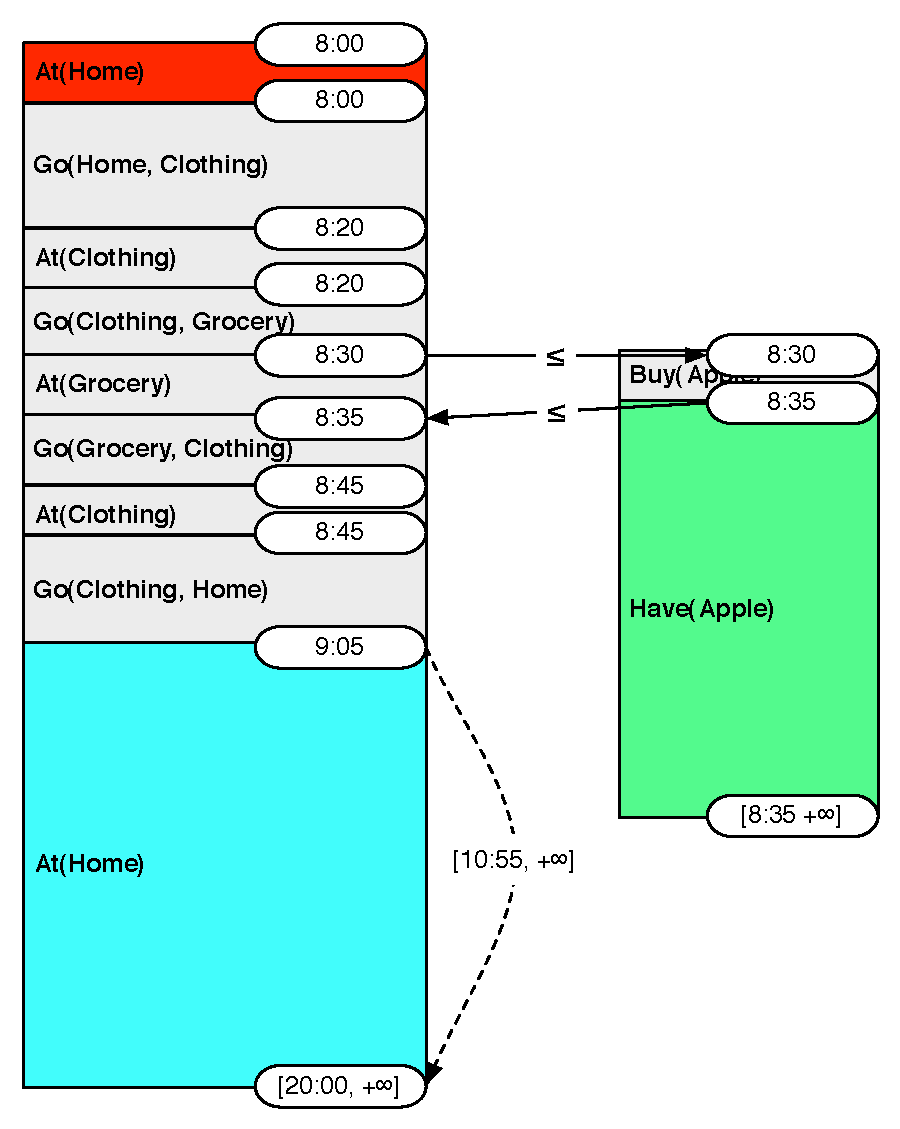
\includegraphics[width=0.65\columnwidth]{figs/example_early}
  \vskip-3mm
  \caption{\small A proactive solution for the plan from
    Fig. \ref{fig:ex:plan} resulting in a Surfacing event at the end
    of mission lasting in excess of $7$ hours.}
  \label{fig:ex:proactive}
\end{figure}

Analyzing the objectives we note that these divergent policies are
because of divergent goal semantics. While visiting {\em Vent 1} was
reflecting a \emph{scientific need}, the goal to be back at the
surface was more of an \emph{operational requirement} to avoid risk
due to the battery running out. While fulfilling both goals are
equally important for mission success, they do not carry the same
notion of {\em urgency}. It is desirable for the AUV to visit vents as
early as possible but there is no strong motivation to return to the
surface before the end of the day. Therefore, a more balanced policy
would be to alternate between the two different approaches depending
on what objective(s) the next action contribute to. The AUV could have
been {\em proactive} until it starts to survey {\em Vent 2} and then
{\em defer} heading back to the surface, continuing to survey the same
area, until it either receives a new goal or the latest start time of
the {\em Go} to \emph{Vent1} action is reached ($\sim$ 17:50). In the
event of a new goal,
% or it is
% really time to go back to the {\em Surface} (around 18:00). Therefore
% when the AUV receive the new objective to sample {\em Vent 1} it would
% be still underwater and will just need to alter its plan to go in this
% new location. 
the resulting mission scenario would then be more efficient in terms
of its \emph{makespan}. Our approach revolves around mission
objectives to be marked as either {\em urgent} or not leading to the
exploration of the plan structure during plan execution to identify if
the action is linked to an {\em urgent} goal -- in which case it need
to be executed {\em proactively} -- otherwise leading towards a {\em
  deferred} execution policy for the action.
 

% We demonstrate a scenario where the AUV ideally uses the two
% approaches at different times. The initial problem is illustrated in Figure
% \ref{fig:Example}.

% The AUV mission starting at 8 AM needs to {\em sample vent2} and
% return to the {\em ship} by 8 PM. The AUV starts traveling immediately
% to {\em vent1}. Considering that that it takes one to two hours to go
% from the {\em Surface} to {\em vent1}, roughly ten minutes to go from
% {\em vent1} to {\em vent2}, and more than two hours in order to {\em
% survey} and {\em sample}, a general plan solution is presented in
% Figure \ref{fig:ex:plan}. The plan presented here is partially
% instantiated giving the AUV the freedom to decide {\em when} to start
% each action within the valid boundary of the solution. For example,
% the AUV should go early in order to {\em sample vent2} so that the
% scientists have the a possibility for requesting more
% tasks. Conversely, heading back to the surface early would waste
% valuable time, roughly two hours, if the scientists decide they want to
% {\em survey} another location. Though by 6pm, it should go to the
% surface so the scientists can pick it up by 8pm. In this scenario, we
% see that the AUV alternated between deciding to execute actions early
% or {\em defer} them depending on the nature of the action it needed to
% take next, or more accurately the nature of the objectives related to
% this action. The AUV was {\em proactive} on traveling to {\em sample vent2}
% because the scientists want it to be completed. On the other hand, the
% AUV has to return to the surface by 8 PM, however, the scientists don't
% explicitly want this done, allowing it to procrastinate.  By
% doing so, the AUV is available to complete new tasks given to it by
% the scientist.\fcomment{One concept that would help if introduced is
%   around the same notion of task span in plan optimization : we have
%   the same problem here but we use a more refined execution policy in
%   order to avoid extraneous actions should a goal come back to us.}



% While this example may appear academic at first, it reflects situations
% we have seen within embedded agent execution in our domain. Indeed, we
% do daily operations wehere our AUV is deployed and scientists can
% remotely send new objectives as the mission goes along to the vehicle
% as they see new areas of interest. Especially in the upper water
% column the nature of the area to be examined depends highly on the
% dynamic of the ocean itself and is difficult to predict beforehand. Therefore,
% scientist can use data sampled by the AUV or other sources (eg
% satellite data, ship based observations, \dots{}) during the beginning of
% the operation in order to give it better informed objectives for the
% rest of the operation. At the same time the vehicle has
% also operational objectives such as going to a place where its
% recovery will be easier for operators. This gives a similar
% distinction between the science objectives and operation
% objectives. Similarly to our example we do not really want the
% AUV to get back to recovery area too early as a new science goal could
% be sent to it which in turn would rather be fulfilled as early as
% possible.

% This paper discusses the problem of dispatching when trying to execute
% a plan. In particular, dispatching in a dynamic environment where the
% plan is expected to change due either to unanticipated events or external
% requests with new directives. External requests  can occur
% at any time which make them in essence uncontrollable events.
% Specifically, we focus on how these new requests, coming from the
% external world, alter the way we need to dispatch the plan, rather than
% how they will be integrated into the plan or any part of the planning
% process. The reason for our separation from planning is that
% oftentimes planning and executing are split up into two different
% jobs. Often times a robotic agent is given an already created plan, and it
% must then choose when to execute parts of the plan. Therefore, our focus is on
% developing a method for dispatch a plan, after it has already been created, while
% understanding that new requests may come in the future.

% The approach we have taken on dispatching looks at the token level of a plan,
% specifically at tokens generated from external requests which we define as goals.
% Because they have been requested by an external person with the intent of being 
% completed promptly, they have a high priority. In contrast, there are tokens that only describe the
% evolution of a timeline, which we define as non-goals. In order to keep the plan 
% valid, the agent is obligated to complete the non-goals, but there is no rush. Thus, the
% non-goals have a low priority. Therefore, we want to complete the goals
% as early as possible in order to give adequate time for the possibility of new
% goals, and complete the non-goals as they become necessary for the validity of the plan. 
% Some may argue that finishing the goals early doesn't guarantee that
% there will be enough time for new goals, however, that is an issue with planning, 
% and our concern is whether dispatching caused the waste of time.


%%% Local Variables: 
%%% mode: latex
%%% TeX-master: "aaai13"
%%% End: 


\section{Previous Approaches to Dispatching}

% \fcomment{I need to rework this as it is not really a state
%   of the art in the current form ... we also need to present that fact
%   that not that much people do consider postponement of actions
%   ... except maybe for dynamic controllability problem ... this may be
%   the key for this part. WE can present proactive approaches as being
%   the general agreement except for the special case of dynamic
%   controllability where 3DC+  introduces wait actions which in fact put
%   time-points that need to be deferred. We on the other hand try to
%   look at another aspect that may trigger the decision to defer an
%   actions based on its purpose}

Dealing with plan execution is not a new problem and we can find a lot
of work that relates to this over several decades. Still, it is
pretty rare to see work that envisage that actions could be
postponed except when this is necessary to not break the current
plan. 


The most prominent work is related to the dispatchability of simple 
temporal networks (STN) \cite{mus98a}. The core of the problem is to
ensure that the temporal constraints can be propagated efficiently
within the plan in order to allow the executive to decide quickly
whether an action should be started or not while ensuring the plan
consistency. In order to accomplish such a task, the STN supporting
the plan to be dispatched is transformed into a All-Pairs network and
stripped of unnecessary edges, often resulting in a more compact
temporal network that lessens the propagation cost of updates. The
role of the executive is to select time-points within the current
execution bounds and propagate its value within the simplified
network. Still, while this work contribute to ensure that execution
time are correctly propagated within the plan with a limited cost, it
does not directly address how to decide what value should be set for a
given time-point in the scope of its possible values. More specifically
it is still the role of the executive to decide whether it should
start an action as early as possible or consider it as not urgent. 

When dealing with least-commitment planning solution this decision is
deferred to the plan executive. For example in \cite{mus98c}, the 
executive is defined as having two responsibilities: the selection and scheduling of plan
events for execution. The executive needs to
be highly reactive as it is necessary to function in a real-time
environment. One solution offered for dispatching events efficiently
is the proactive approach. This approach greatly reduces the plan
flexibility, and therefore robustness, as all start time-points are
grounded to a specific value which is compatible with the initial
constraints. % In order to avoid having a procrastinating system the
% overall agreement in term of policy is to start an action as early as
% possible (ref ?). 

% \fcomment{Therefore, one reoccurring problem of dispatchability is finding a way
% of balancing efficiency, proactive, with flexibility,deferred.}
\fcomment{We need to update this to reflect that it is not ETS}
%There have been many uses of these two approaches when dispatching plans, as
%previously shown, but a compromise to one is most often used rather than
%a balance. Demonstrated in the tool MAPGEN \cite{bresina03} which used
%the Earliest Time Solution (ETS) for generating and displaying plans
%very quickly. Then allowing the users to manipulate the plan afterwards,
%getting around the problem of ETS generating undesirable plans. What is
%needed is a way of using both proactive and deferred together giving a
%balanced approach to dispatching.

While in the common case this might be acceptable it
may become problematic when put in he context of potential new
objectives emerging during the mission.  Take our AUV example,
and apply the proactive approach globally --- assuming that all actions
can be completed on their minimum time.  As shown in 
Fig. \ref{fig:ex:proactive}, the proactive approach allows the
AUV to {\em Sample Vent2} before noon but as continue through
the plan it results in the AUV getting back to the {\em Surface}
by 12:21 and being stuck in the context of the current plan for the
next 7 hours and 39 minutes. Should the scientist want to {\em Sample Vent1}
the AUV will then be forced to re-plan accordingly and
go back and forth between the surface and the locations all other
again. By being blindly proactive, the AUV made its overall strategy
less efficient than if it took the option to procrastinate at {\em Vent2}
until it needs to get back to the surface. 


\begin{figure}
  \centering
  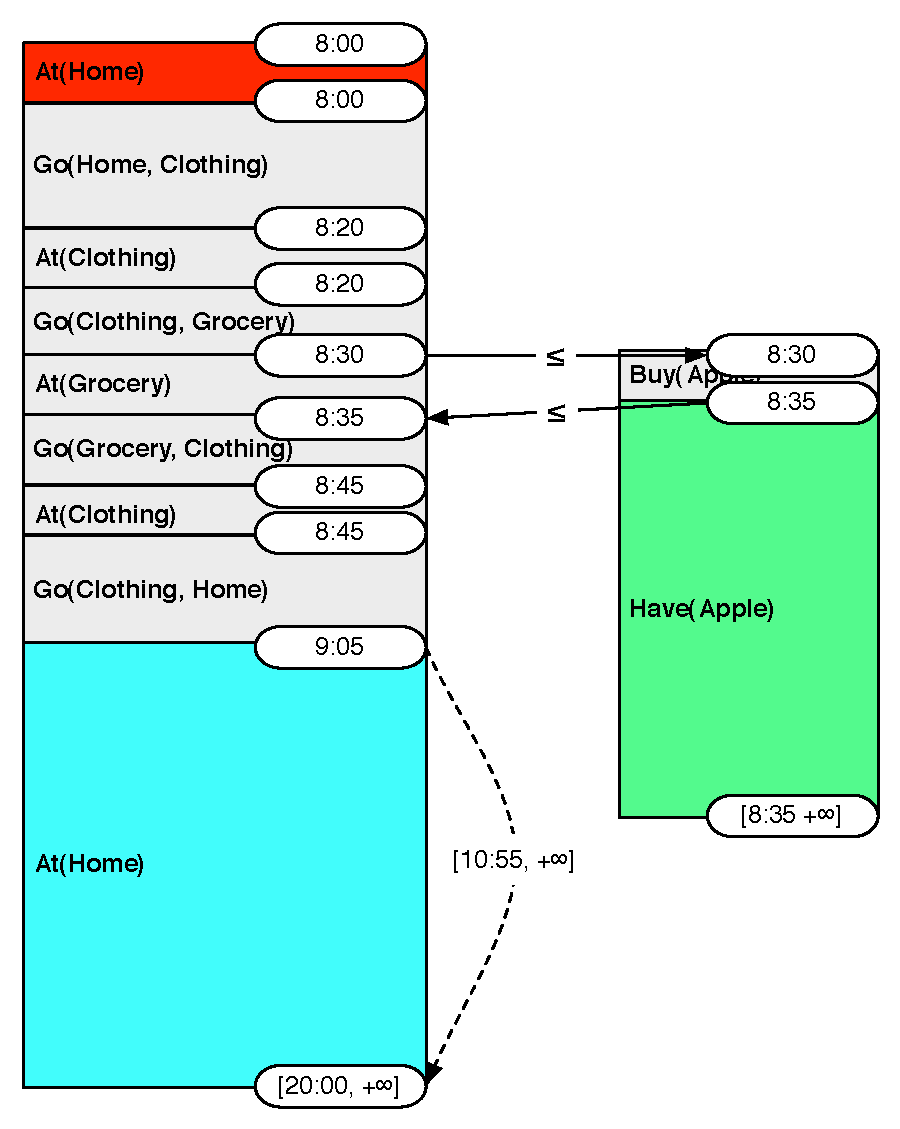
\includegraphics[width=0.65\columnwidth]{figs/example_early}
  \caption{\small A proactive solution for the plan from
    Fig. \ref{fig:ex:plan} resulting in a Surfacing event at the end
    of mission lasting in excess of $7$ hours.}
  \label{fig:ex:proactive}
\end{figure}

One case we have seen in literature where a time-point is
considered to be deferred is related to the dynamic controllability
issue with STNs with uncertainty (STNU). In \cite{morris01}, they propose 
an algorithm that during planning insert wait constraints within the
solution temporal network that will allow one time-point to wait until
an uncontrollable event occurs. In this case, the deterrence of the
execution of this time-point is enforced in order to ensure robust plan
execution despite exogenous uncontrollable events. In
\cite{gallien2006},  this approach is further discussed along with the
Makespan issue while dealing with least-commitment planners which can
insert unjustified waits within the plan potentially decreasing in turn the
overall performance of the system. Both of these approaches show that
when dealing with uncontrollable temporal constraints -- such as for
example the duration of a navigation task which depends on external
factors -- it is necessary to defer some actions in order to ensure
the plan execution. 

An alternative approach is related to work with soft constraints
within the temporal domain indicating preferences on actions timing
such as in \cite{khatib2001temporal}. This should provide  a general
solution for users to specify whether actions of the plan should be
preferably started. One problem with general frameworks dealing with
soft constraints though is their poor performances \cite{bartak2002}
as the general problem is NP-hard. Even though it can be reduced to a
more tractable (polynomial) solution by specifying preferences as
convex functions \cite{rossi2006learning}, the  
complexity is still cubic in relation to the number of
variables. Moreover the solutions proposed do optimize the plan {\em
  a-priori} reducing then the plan flexibility which in turn makes it
more prone to failure during execution.

Our work is complementary to much of the previous work.  While we do
not explicitly deal with dynamic controllability, our approach is not
inconsistent with that work.  In any case, our focus is not on the
observation of events during execution but rather on the possibility
of new objectives arising at any time, and we want to avoid doing
actions that are not ``urgent'' in order to preserve the context for
those objectives.  Similarly, we have not implemented temporal
preference specification during planning, which has the effect of
limiting execution-time flexibility.  Our intent is to defer temporal
decisions to the executive allowing it to adapt the plan to new
objectives without heavily relying on plan-repair or re-planning
solutions that could badly impact system reactiveness.


% Our work on the other hand is more complementary to previous work, indeed
% while we do not really deal with dynamic controllability in our
% problem -- which can anyway be treated as in this previous work -- the
% core of our problem is not that much the observation of events during
% execution (which is more a observation related impact) but instead we
% are more focused on the knowledge that, within our agent, new
% objectives can emerge at any time, and we want to avoid as much as
% possible doing actions which are not ``urgent''. Similarly, while we do
% not really deal with complex preferences specification that can help
% improve the planned solution our purpose is to defer the decision to
% start to execute actions within the plan to the executive allowing to
% quickly adapt the plan without heavily relying on plan-repair or
% re-planning solutions that could badly impact the system reactiveness.
% By doing so, we take the risk of doing unnecessary actions as new
% goals need to be integrated in the plan.

% s
% considered to be deferred is related to the approach proposed in 
% \cite{morris01} to deal with dynamic controllability issue. 
% \fcomment{following will be included in former para. Also we need to
%   address that it is in fact outside of our scope here ... we actually
% do not address dynamic controllability, worse we tend to make waiting
% actions more brittle in general as we take the upper bound  for needed
% actions}

% The only work where we see 

% % Dispatchability for a simple temporal network (STN) has been identified
% % with whether a plan is capable of fast execution, retains its
% % flexibility despite uncertainty in the plan, and all information is
% % available at execution \cite{mus98}.  To accomplish the task of
% % efficient execution, the STN's are transformed into All-Pairs networks
% % and striped of their unnecessary edges, which will often create a more
% % compact temporal network and esse the propagation of its updates.
% % The executive then selects a timepoint, within the bounds of the 
% % execution time, and every timepoint before it has
% % already been executed. It then sets the start time to the selected
% % timepoint and propagates the needed changes throughout the graph
% % \cite{mus98}. The process of selecting a timepoint can lead to
% % issues when two timepoints have the possibility of being executed at the
% % same time, where one should necessarily come first, but the incorrect
% % one gets selected first. This mistake can cause the STN to become
% % brittle, which leads to a higher chance of failure in the plan.

% % \fcomment{Need to continue to refine from here and talk about STNU and
% %   morris01 as  the only approach we know of where postponed events are present
% %   though the inserted wait}

% % Take our shopping example\fcomment{figure again}.  We'll say the agent wakes up
% % at 9 AM and the duration for traveling to the store is forty minutes
% % and buying the apples is ten minutes. Using the proactive approach, the
% % agent will start shopping as soon as possible and thus be done shopping
% % by 10 AM. The agent will then go directly home afterwards to satisfy the
% % ``home by 8 PM'' goal. However by doing so, the agent will be back
% % home by 11am with the constraint to stay at home for the next 9
% % hours. 
% % \fhighlight{If his wife} is then calling to ask him to buy extra things it will
% % results on hime to need to fully relax his current plan and go back
% % and forth between its home and the store all other again. By being
% % fully proactive the agent.\fcomment{Maybe what was meant initially
% % here is more related to dynamic controllability which mean that I need
% % to twek this text to be more related to a modelled
% % but uncontrolbale situation.}


% % However, the start time for this goal will be roughly
% % 11 AM, and if the agent wants to get some dessert before dinner it will
% % cause a failure in the plan. What this example shows is how EST can
% % severely reduce the flexibility of a mission. EST can also cause
% % inconsistency within the plan.

%  {\em \fhighlight{Therefore,} \cite{mus97}\fcomment{See comment before} added
% implied links between timepoints allowing the planner to find them
% efficiently.\fcomment{I don't get what you mean here}}


% Another issue with execution is uncertainty in the plan. The above
% example illustrates the uncertainty about when the agent should go home
% or if the agent will want to buy more food during the mission. A
% solution for execution uncertainty is the least-committed method, which
% waits until that last moment to execute events. This approach keeps the
% plans flexibility and it allows the executive to have all of the
% available information before making a choice (Block, 2006). However, it
% has been argued that the least-committed method is an inefficient
% solution because in a real-world environment an agent might idle for
% long periods of time (Gallien, 2006). This can severely decrease the
% overall performance of the system. Lets demonstrate the least-committed
% policy in our Shopping agent example using the same goals and durations
% as before. This time around the agent won't want to do anything until it
% is absolutely necessary to do it. The agent will then wait until 6:20 PM
% before leaving and will finish shopping at 7:20 PM this way the agent
% can be home by 8 PM. However, even though this keeps flexibility in the
% plan there are a few issues. If there happens to be traffic then the
% agent might not make it home by eight PM. Also the agent procrastinates
% all day just waiting to go shopping rather than starting early on in the
% day, which wastes valuable time. Their (Gallien, 2006) solution is to
% change the planning heuristic altering how their plan is created
% inevitably adjusting it for faster execution.


%%% Local Variables: 
%%% mode: latex
%%% TeX-master: "aaai13"
%%% End: 

 
\section{Planning Definitions}
\label{sec: defs}

The focus of this paper is on the possibility of \emph{new objectives}
arising at any time with consequent need to avoid doing actions that
are not ``urgent'' in order to preserve the context for these
objectives. Our robot generates and dispatches a partial plan in
continuum to a lower level controller which further decomposes these
plans towards atomic actions. These actions ultimately actuate
hardware on our AUV; the world responds by sending sensory feedback as
\emph{observations} up thru the hierarchical controller
\cite{mcgann08bdup,rajan12dup}. Details of the controller are beyond
the scope of this paper and are omitted without loss of generality of
the concepts described.

We first consider some basic representational definitions related to
temporal planning consistent with \cite{Nau:2004}:

% To consider the overall planning and plan execution within an agent we
% use the definition of a temporal domain, planning problem and solution
% as provided by \cite{Nau:2004}:

\begin{definition}
  \label{def:domain}
  A temporal planning domain is a triple $D = ( \Lambda_\Phi, O, X )$, where:
  \begin{itemize}
  \item $\Lambda_\Phi$ is the set of all temporal databases that can
    be defined with constraint, constant, variable, and relation
    symbols in the representation.
  \item $O$ is a set of temporal planning operators.
  \item $X$ s a set of domain axioms.
  \end{itemize}
\end{definition}

A \emph{token} is a property that holds within a flexible temporal
interval which represents an action or a state associated with $O$ or
$X$ \cite{py10dup}. The temporal interval is delimeted by two 
{\em timepoints} marking the possible values of its {\em start} and
{\em end}.
 % \kcomment{define observations/timepoints; better
 %  still define the life-cycle within which an observation is received}

\begin{definition}
  \label{def:problem}
  A temporal planning problem in $D$ is a tuple $P = ( D, \Phi_0, \Phi_g )$, where:
  \begin{itemize}
  \item $\Phi_0 = (F, C)$ is a database in $\Lambda_\Phi$ that
    satisfies the axioms of $X$.  $\Phi_0$ represents an initial
    scenario that describes not only the initial state of the domain
    but also the evolution of the world as depicted by the
    observations fed by the executive in the course of the mission.
  \item $\Phi_g = (G, C_g)$ is a database that represents the goals of
    the problem as a set $G$ of tokens together with a set $C_g$ of
    objects  and temporal constraints   on variables of $G$.
  \end{itemize}
\end{definition}

\begin{definition}
  \label{def:plan}
  A plan is a set $\pi = \{a_1,...,a_k\}$ of actions, each being a
  partial instance of some operator in $O$.  We define $\lambda$ as
  the state-transition function.  $\pi$ is a solution of a problem $P
  = (D, \Phi_0, \Phi_g)$ iff there is a database in $\lambda(\Phi_0,
  \pi)$ that entails $\Phi_g$.
\end{definition}
 
Our focus is on executing plan $\pi$; however, to reflect the dynamic
interaction of the agent with its environment we need to refine the
definition of the sets $\Phi_0$ and $\Phi_g$. As the world evolves,
new (or refinement of existing) observations are added to
$\Phi_0$. Similarly, the agent operator can request new future goals
to be added to the agent $\Phi_g$ as mission time advances. We note
$\Phi_0(t)$ and $\Phi_g(t)$ the value of these sets at the instant
$t$. For the sake of simplicity we consider that the alteration of
these sets is purely additive with time\footnote{In practice, their
  evolution is more complex as completed goals becomes observation;
  even a goal previously requested can be cancelled by the
  operator. While this assumption largely simplifies problem
  description, our algorithm works regardless.}:
\[ \forall \{t, t'\}: t \le t' \Rightarrow \Phi_0(t) \subseteq \Phi_0(t')
\wedge \Phi_g(t) \subseteq \Phi_g(t') \] 

%\fcomment{I will need to refine this and make it more convincing}
The dynamically growing nature of $\Phi_0$ reflects the cumulative
observation as the agent execute its plan $\pi$. In nominal situations,
new elements of $\Phi_0$ are refinements of the plan -- for example by
asserting that a planned command just started\footnote{This precludes
  situations where new observations invalidate the plan; this is out
  of the scope of this paper}. The agent can also receive new
objectives at any point with those added to $\Phi_g$. This assumption
has an impact on how it is preferable to handle plan execution. Indeed
while deciding when to start an action within the plan, one need to
make sure that the execution of this action will not limit the ability
of the agent to treat potential future emerging goals. In the light of
it the agent should at the best of its knowledge try to balance the
impact of the next available action as early as possible or prefer to
delay it in the eventuality new goals occur. In our example, it was
making sense to go to Vent2 early, but on the other hand going back to
the surface too soon would result in locking the AUV -- within its
current plan -- at the Surface until $8$ pm. The solution providing
the most flexibility for the AUV was therefore for it to alternate
between the two policies depending on the action impact.

In order to help the AUV have a better knowledge on the nature of the
goals we do consider that each goal provide information on its
priority. In that purpose, we define that $\Phi_g$ is partitioned into
two sets:

\begin{itemize}

\item the \emph{internal} goals $\Phi_{gi}$ which represent goals the
  agent {\em needs} to maintain internally. These goals will be
  considered as objectives that are not of the higher priority and
  therefore their actions can be deferred during execution.

\item the \emph{external} goals $\Phi_{ge}$ which represents the goal
  received by the agent externally. As these goals are requested by
  the user, we consider them as to be of higher important -- ie the
  agent {\em wants} to execute them. Therefore, their execution should
  be preferrrably proactive.

\end{itemize}

At any point we need to evaluate an action within our plan $\pi$ we
consider that this plan is up to date and provide a solution of all 
the goals of both $\Phi_{gi}$ and $\Phi_{ge}$ that can reasonably be
done within the current mission scope.

\section{Algorithmic Description}

As a new action can be dispatched for execution, the executive needs
to evaluate how it relates to the goals of the plan. Intuitively if
this action was generated by (or contributes to) an internal goal of
$\Phi_{gi}$ it needs to be taken proactively, while otherwise we can
consider it as non-urgent. Therefore, when evaluating if the token
representing this action within the plan the executive needs to do a
forward search on the causal links related to this token to see if
they lead to an internal goal as implemented in Algorithm
\ref{DispatchToken}.

\begin{definition}
\label{def:subgoalLink}
A goal $g$ is causally linked to a state value $c_i$ if there is an
action such as $g$ is an effect of this action and $c_i$ is one of its
conditions\footnote{For metric temporal plans, Allen Algebra
  \cite{allen84} is the basis for determining relationships between
  actions and is more general than pre-conditions in classical
  planning.}. 
% A causal link is defined as linking a goal as an effect of an action
% whose conditions are needed in order to complete the goal and, thus, are
% subgoals. This link can be recursive as the conditions themselves may
% be the effect of an action causing a causal chain to build.
\end{definition}

As a result all the conditions of this action can be assumed to be
subgoals with similar priority as $g$.

\begin{algorithm} [H]
  \caption{\small The function $DispatchToken$ finds if there is a
    goal in $\Phi_{ge}$ that is connected to the token, $t$, and, if
    so, dispatches the token.}
\label{DispatchToken}
\begin{algorithmic}
\small 
\Function{DispatchToken}{Token $T$}
\State Boolean $Goal = \textsc{SearchForGoal}( T )$
\If{ $Goal$ $=$ True}
	\State \Return Dispatch $T$
\ElsIf{ $T$ start upper bound $ \leq $ current tick}
	\State \Return Dispatch $T$
\Else
	\State \Return Don't dispatch $T$
\EndIf
\EndFunction
\end{algorithmic}
\end{algorithm}

\begin{algorithm} [H]
  \caption{\small The function $SearchForGoal$ does a Forward search
    looking for a token that is in the set $\Phi_{ge}$.}
\label{SearchForGoal}
\begin{algorithmic}
\small
\Function{SearchForGoal}{ Token $T$ }
\If{$T \in \Phi_{ge}$}
  \State \Return True
\Else 
  \State List $Fringe$ = \{ Actions that $T$ is Condition of \}
  \ForAll{Action(s), $A$, in $Fringe$ }
     \ForAll{Effects, $E$ of $A$}
       \If{$E \in \phi_{ge}$}
          \State \Return True
        \Else 
           \State List $L$ = \{ Action(s) that $E$ is Condition of \}
           \State $Fringe$ = $Fringe \cup L$ 
        \EndIf
      \EndFor
  \EndFor
\EndIf
\State \Return False
\EndFunction
\end{algorithmic}
\end{algorithm}

This Algorithm is the central deciding point for how a
token should be dispatched. By finding out that a token is connected
to a goal in $\Phi_{ge}$, we conclude that the token is a sub-goal,
and thus dispatch it immediately being proactive.  On the other hand,
if the token is not connected to a goal then we defer dispatching it
until necessary.  This demonstrates our distinction between how we
dispatch tokens, proactive or deferred.

A crucial part for deciding how to dispatch a token is finding whether
the token in question is connected to a goal in $\Phi_{ge}$, call it
$G$. Algorithm \ref{SearchForGoal} does the function of searching for
$G$ in a forward-search manner. We define a causal link within our
plan that must be met in order for our search to function.

During our search, if we find $G$ then we know that the original token
is part of the solution for completing $G$.  As such, we want to be
proactive with completing the token early so as to ultimately complete
$G$. If we don't find $G$ then the token has no connection to an
external request. The token still needs to be dispatched, however,
there is no one explicitly requesting it to be accomplished. Thus,
there is no reason to be proactive.

This algorithm is equivalent to a breadth first search along the
planning structure starting from the action we need to
evaluate. Therefore, its complexity is $O(N+E)$ where $N$ is the
number of tokens within the plan and $E$ the number ofcausal links that relate
these tokens. 

%\subsection{Dynamic solution during planning}
%
%Searching for a goal as Algorithm \ref{SearchForGoal} does can be
%quite computational expensive particularly if there are many tokens
%that are continuously being dispatched. Completing a full search every
%time a token needs to be dispatched can severely slow down the
%execution process, which needs to remain quick to ensure proper
%execution. Therefore, our next algorithmic approach distributes the
%full search within the creation of the plan.  Resulting in spreading
%out the full cost of the search. In order to not repeatedly search the
%plan, we save the tokens that are connected to a goal in $\Phi_{ge}$
%found during the search. In this way, we acquire a list of tokens,
%$List_{goals}$, that should be dispatched early.
%
%An alternative solution is to embed the propagation of these value
%during the planning search. The algorithm uses the same dispatching
%method as algorithm \ref{DispatchToken}.  The difference is that
%rather than searching for the goal using algorithm
%\ref{SearchForGoal}, it only searches the list, $List_{goals}$, to see
%if the token is in it. The actually searching for the goals and
%causally connected tokens happens in algorithms \ref{NotifyActivated},
%\ref{NotifyMerged}.
%
%\begin{algorithm}[H]
%\caption{\small Saves goals as they are added to plan}
%\label{NotifyAdded}
%\begin{algorithmic}
%\Function{NotifyAdded}{ Token $T$ }
%\If{$T$ is a Goal in $\Phi_{ge}$}
%	\State Insert $T$ into $List_{goals}$
%\EndIf 
%\EndFunction
%\end{algorithmic}
%\end{algorithm}
%
%\begin{algorithm} [H]
%\caption{\small Removes the token after it is removed from the plan}
%\label{NotifyRemoved}
%\begin{algorithmic}
%\Function{NotifyRemoved}{ Token $T$ }
%	\State Remove $T$ from $List_{goals}$
%\EndFunction
%\end{algorithmic}
%\end{algorithm}
%
%\begin{algorithm}[H]
%\caption{\small Searches for tokens connected to goals}
%\label{NotifyActivated}
%\begin{algorithmic}
%\Function{NotifyActivated}{ Token $T$ }
%\If{$T$ is a goal in $\Phi_{ge}$ or $T$ is linked to a goal through one causal link}
%	\State Recursively search the reverse causal link and add the tokens into $List_{goals}$
%\EndIf
%\EndFunction
%\end{algorithmic}
%\end{algorithm}
%
%\begin{algorithm}[H]
%\caption{\small Deactivates token in plan}
%\label{NotifyDeactivated}
%\begin{algorithmic}
%\Function{NotifyDeactivated}{ Token $T$ }
%\If{$T$ is not a goal and not one causally linked to a goal}
%	\State Remove $T$ from $List_{goals}$
%\EndIf
%\EndFunction
%\end{algorithmic}
%\end{algorithm}
%
%\begin{algorithm}[H]
%\caption{\small Searches plan when tokens are merged}
%\label{NotifyMerged}
%\begin{algorithmic}
%\Function{NotifyMerged}{ Token $T$ }
%\If{$T$ is goal in $List_{goals}$}
%	\State Recursively search the reverse causal link of the active token merged with $T$ and add tokens to $List_{goals}$
%\ElsIf{The active token of $T$ is in $List_{goals}$}
%	\State Recursively search the reverse causal link of $T$ and add tokens to $List_{goals}$
%\EndIf
%\EndFunction
%\end{algorithmic}
%\end{algorithm}
%
%\begin{algorithm}[H]
%\caption{\small Removes token when split}
%\label{NotifySplit}
%\begin{algorithmic}
%\Function{NotifySplit}{ Token $T$ }
%\If{$T$ is not a goal or not one causally linked to a goal}
%	\State Remove $T$ from $List_{goals}$
%\EndIf
%\EndFunction
%\end{algorithmic}
%\end{algorithm}
%
%In order to distribute the search, we situate our algorithm within the
%planning search of the Europa Planner,\cite{frank2003}, which offers 
%callback functions for when a token in the plan is altered. The majority
%of the searching happens when tokens are either activated or 
%merged. For a token to merge with another token it has to be compatible with
%another token already in the plan. Splitting happens when they are
%no longer compatible. We have designed our algorithm around the
%Europa Planner, however, we believe that the general approach
%can work on any other planner. 
%
%Taking full advantage of the planning search, we
%use a backwards search from the goal following the reverse causal link
%to the connected tokens.  We fully search from the goals because we
%know that all the tokens connected through the causal link are
%sub-goals. By contrast, fully searching each token could be
%wasteful because there is no certainty that it will be linked to a
%goal and, therefore, could bring little value to our search. However,
%some tokens may get added to the plan or linked to a goal after we
%have already searched the goals. Therefore, for every token we do a
%local forward search of one causal link to verify if it is connected
%to a goal in our saved list.  If so, we do a full backwards search
%from the token since it has now proven to be valuable. After the plan
%has been searched, it is as easy as searching a list for a token to
%see if it should be dispatched early or be deferred to later.
%
%This approach is potentially more costly than the previous algorithm 
%as it needs to do local updates whenever the plan is altered by the search
%including retracting past updates if a backtrack occur during the
%search. Still it is compelling in the fact that this cost occurs during
%planning reducing the decision problem during execution to simply
%check if the given action has been marked during planning. It has
%been the solution we have preferred within our system for this reason
%as it is functionally equivalent to previous algorithm while reducing
%extra computation cost as the plan is executed. Planning phases occur
%within the plan only when either the initial plan failed to execute or
%the set of goals has been altered. Therefore, it is safe to assume that
%planning should occur more sporadically than execution decisions 
%which then give an edge to this latter algorithmic solution. 

%%% Local Variables: 
%%% mode: latex
%%% TeX-master: "aaai13"
%%% End: 


\section{Experiments}
\label{sec:exp}

The experiments follow a mission similar to the original plan given in
Fig. \ref{fig:ex:plan}. The AUV needs to {\em Sample Vent2} and return
to the {\em surface} by the end of the mission. The AUV must also be
at the {\em surface} around
13:00. % with plans being produced by the europa planning engine
% \cite{frank2003}.
Fig. \ref{fig:ex:mixed1} demonstrates the resulting plan after
processing by Algorithm \ref{alg:dispatch} using our executive \rx
which synthesizes temporal plans.

\begin{figure}[!htbp]
  \centering
  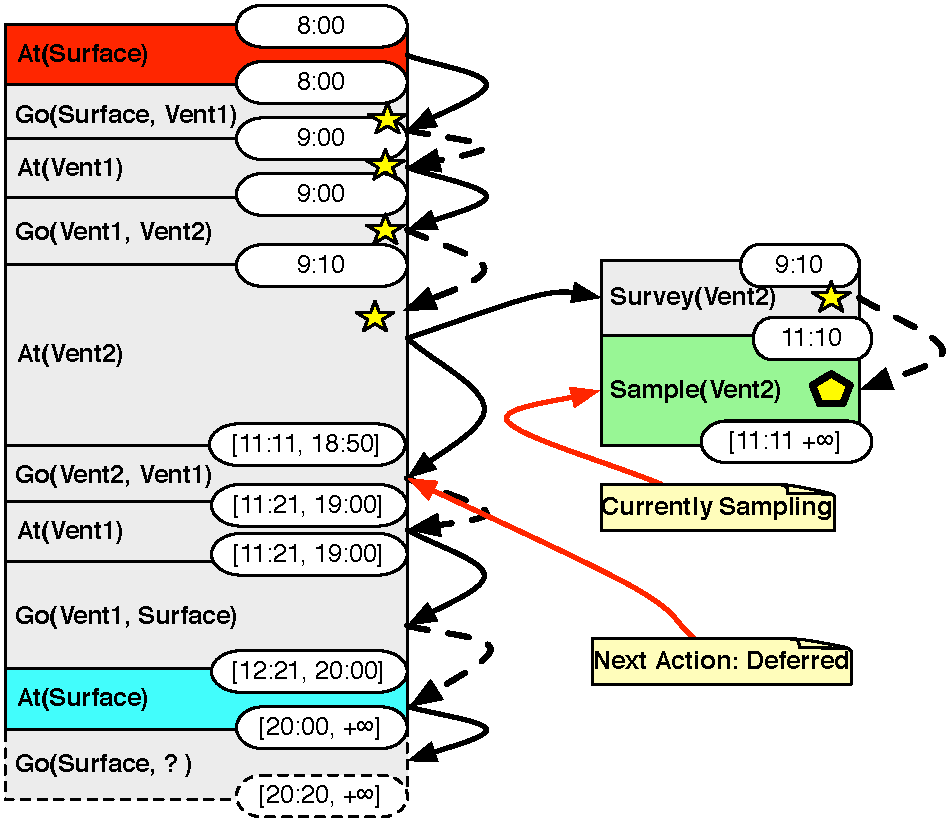
\includegraphics[width=0.9\columnwidth]{figs/example_MixedInitial}
  \vskip-2mm
  \caption{\small Solid lines indicate conditions and dashed lines
    indicate effects. Pentagons indicate {\em urgent} goals and stars
    indicate tokens that were deduced as {\em proactive}.}
  \label{fig:ex:mixed1}
  \vskip-3mm
\end{figure}

% For Algorithm \ref{SearchForGoal}, the search is straight forward. For
% example in 

% As shown in Fig. \ref{fig:ex:mixed1}, if the AUV is {\em At Surface}
% at execution time, the next {\em Go} token will be dispatched. Because
% the search follows causal links, it will encounter the {\em Sample
%   Vent2} goal resulting in dispatching proactively.  Similarly, this occurs
% for all of the tokens that are starred. The next token that is not
% starred, {\em Go(Surface)}, is continuously searched but deferred,
% because it is not connected to an urgent goal. The resulting AUV stays
% at {\em Vent2} rather than heading to the {\em Surface} immediately.

As in Fig. \ref{fig:ex:mixed1}, the AUV is {\em At Surface} initially.
At execution time, the next {\em Go} token will be dispatched
proactively, because when the search follows causal links, it
encounters the urgent {\em Sample Vent2} goal.  This occurs similarly
for all tokens that are starred. {\em Go(Surface)} is deferred,
because it is not connected to an urgent goal using forward
search. Consequently, the result requires the AUV to stay at {\em
  Vent2} rather than heading to the {\em Surface} immediately.

%For the distributed algorithm approach, each token is checked during
%the creation of the plan to see if it is an external goal in
%$\Phi_{ge}$, or connected to one through a causal link. When the {\em
%Sample Vent2} is checked, we immediately find that it is a goal. We then
%follow the reverse causal link and find {\em Survey Vent2}.  However to
%better illustrate the algorithm, we can imagine that only the {\em Survey
%Vent2} has been causally connected to the goal so far. Therefore, we
%only star those two tokens. The path from {\em Surface} to {\em Vent1}
%to {\em Vent2} has yet to be built. When the path has finally been
%built, and {\em At Vent2} is checked, our algorithm searches one
%causal link and finds {\em Survey Vent2} which is starred. The search
%then follows the reverse causal link and stars the rest of the
%path. The starred tokens will then be proactively dispatched while the
%non-starred tokens will be deferred until later. Having similar
%results to Algorithm \ref{DispatchToken}.

We then introduced a new {\em urgent} goal to {\em Sample Vent1} at
11:30 with the resulting plan shown in Fig. \ref{fig:ex:mixed2}. Since
there is not enough time to {\em Sample Vent1} and be at the surface
by 13:00, the goal is placed after the AUV visits the
surface. Propagation results in marking the actions which were thus
far deferred are now being causally linked to the new {\em urgent}
goal of {\em Sample Vent1} and their execution status is updated. The
resulting starred tokens get dispatched proactively which includes all
actions related to the mid-day surfacing goal.

\begin{figure}[t]
  \centering
  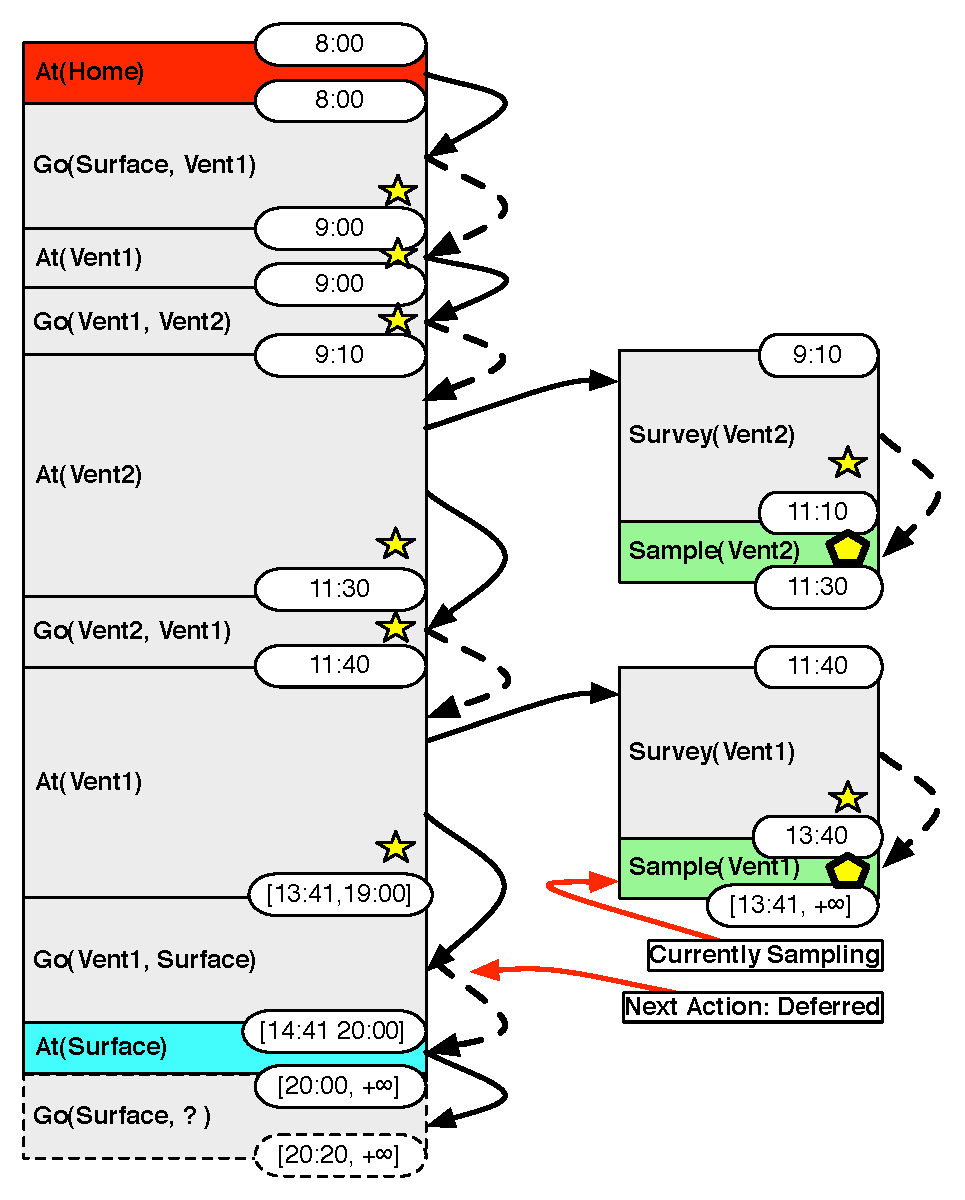
\includegraphics[width=0.8\columnwidth]{figs/example_MixedUpdate}
  \vskip-3mm
  \caption{\small The solution after receiving external request for
    the plan from Fig. \ref{fig:ex:mixed1}}
  \label{fig:ex:mixed2}
  \vskip-3mm
\end{figure}

Meanwhile the actions related to the final surfacing goal remain {\em
  deferred} and won't be executed until 19:00 allowing the vehicle to
sample {\em Vent1} for a duration of 2:50 hours.  After returning to
the {\em Surface}, our planner and domain inserted a partially
instantiated action to {\em Go(Surface, ?)} (dashed in the figures).
This is an artifact resulting from the plan model which specifies that
an {\em At} token is necessarily followed by a {\em Go}.  However, our
algorithm will not be dispatching this token as it is not connected to
an {\em urgent} goal and its upper bound start time ($+\infty$) will
not be met within the scope of the mission.

\subsection{Performance Analysis}

In our experiments, the simulated AUV missions ran on a Linux virtual
machine running on a MacBook Pro allocated one core from a $2.33$ GHz
Intel Core $2$ Duo processor.
% Time was recorded using a thread clock for the most accurate time.
A short mission duration ($200$ seconds) was selected to allow rapid
assessment with multiple runs; increasing mission duration generates
no impact of significance.
% We chose a mission length of 200 seconds to allow simulation to
% be completed quickly. There is, however, no difference in performance
% if the mission were longer as the same plan would be produced just
% with different timepoints.
 
Fig. \ref{fig:example_run} shows a mission run that is similar to the
example in Fig. \ref{fig:ex:plan}.  To increase plan complexity a
total of $8$ intermediate locations were added between the {\em
  surface} and {\em vent 1}, with all evaluations taking less then $1$
millisecond. The largest performance spikes were due to the need to
evaluate the dispatching condition for an {\em At} token which is
followed by a {\em Go} token resulting in two forward searches within
the plan structure. This is because the dispatch window is larger than
the minimum duration of the {\em At} token; since our plan uses a {\em
  Go} immediately after, this \emph{Go} token also needs to be
evaluated.

\begin{figure*}[t]
  \centering
  \vskip-3mm
  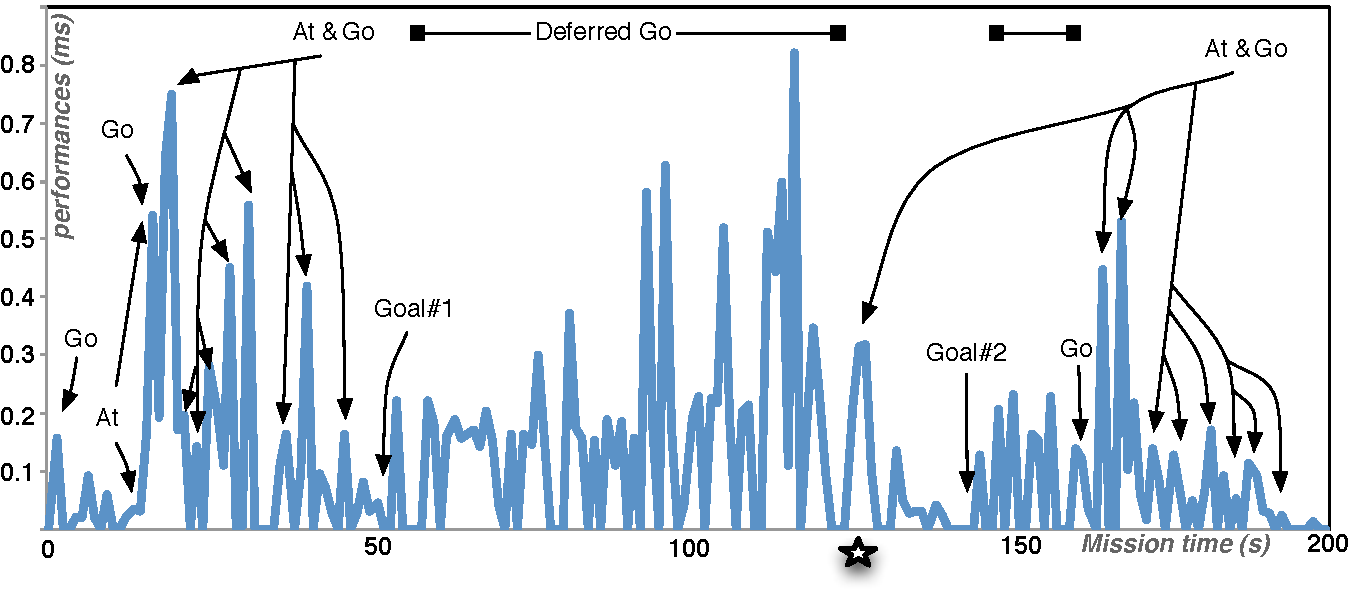
\includegraphics[width=1.2\columnwidth]{figs/example_run.pdf}
  \vskip-2mm
  \caption{\small A mission run that shows the time needed for
    dispatching. The star represents when Goal \#2 is received and
    integrated into the plan. Lines with boxes at the end represent
    the deferred action {\em Go} Because of space, we didn't put an
    arrow to every {\em At}. Our concern were the peaks that showed
    where the system had to dispatch both {\em At} and {\em Go}. }
  \label{fig:example_run}
  \vskip-2mm
\end{figure*}


We also identified a clear trend toward decreasing timing as the agent
comes closer to the completion of either {\em Goal \#1} or {\em Goal
  \#2}. This is correlated to the reduction in search distance toward
these goals as we execute new actions.  We see an important
variability in execution time which is likely due to context switching
between processes and threads within our agent; multiple cores in the
virtual machine is likely to remove this variation.  The bump in
timing between time-step $56$ and the introduction of {\em Goal \#2}
at $127$ is because the algorithm is continuously searching the graph
from the next {\em Go}, which during this period, is not connected to
an {\em urgent} goal. The resulting exhaustive search in the plan
graph during this period is on an average above $0.2$ milliseconds. At
tick $127$, the {\em Go} is no longer deferred and gets dispatched.
% The search for our algorithm execution time {\em Goal \#2} becomes
% relatively simple as it is not very far away in the plan
% \kcomment{from what? from the end of the plan?}, and thus the time
% decreases significantly.

\begin{figure}[!b]
  \centering
  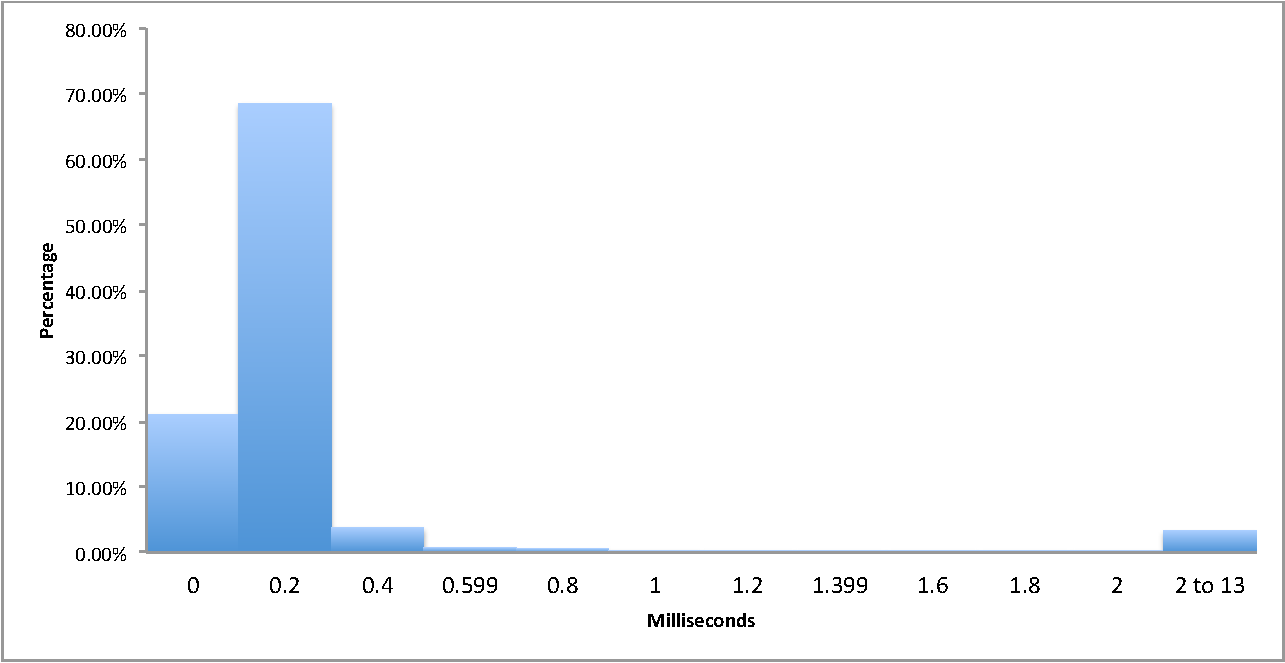
\includegraphics[width=\columnwidth]{figs/HistogramAlg1}
  \caption{\small Algorithm \ref{DispatchToken} was timed at every
    increment ($1$ Hz) for $500$ simulated missions. One goal was
    inserted into the plan at random during the mission. The histogram
    shows the distribution of the time, which is heavily skewed to the
    left.}
  \label{fig:histogram}
\end{figure}

% In order to demonstrate the average amount of time that Algorithm
% \ref{DispatchToken} uses, $500$ simulated missions were recorded and
% timed at every increment of the mission time. 
Fig. \ref{fig:histogram} shows the distribution of execution time for
$500$ simulated missions. It shows that $90\%$ of the time our
algorithm completed its search in less than $0.2$ millisecond. The
distribution is long tailed with the worst performance between $2$ and
$13ms$ occurring for less than $5\%$ of the runs. Such performance is
exhibited when the {\em tokens} evaluated are meant to be {\em
  deferred} which is not critical to the overall execution.

% which makes the small loss of performances not as
% critical.


%%% Local Variables: 
%%% mode: latex
%%% TeX-master: "aaai13"
%%% End: 


\section{Discussion and Future work}
\label{sec:conclude}

Increased robustness in hardware has led to persistence of robots
often in hostile environments such as our oceans. And with onboard
autonomy, the increased versatility has resulted in the need to anticipate
and adapt to goals during mission execution.  Most existing autonomy
approaches fall short of dealing with the ensuing tension of
dispatching temporal actions either proactively or deferring them.
Typically, the solution pursued is to integrate such knowledge within
the system domain description itself which often results in a more
complex model. Our experience shows that such added complexity makes
the planning domain harder to maintain and more error prone,
motivating the approach to provide a simple yet efficient solution to
deduce execution policy based on the supplementary goal information
namely that of {\em urgency}.  The work in this paper focuses on plan
structure in abstraction without direct consideration of timing
constraints applied to each goal in the plan. We are consequently able
to use breadth first search within the existing plan structure to
select different execution policies for each action within the
plan. By doing so, we can improve overall mission execution by avoiding
proactivity that could lead to inefficiency in handling new goal
requests.

A number of open issues remain to be explored, however. The causal
link traversal proposed is agnostic to the temporal constraints
applied to timepoints of the plan; including such information could
greatly increase the quality of our solution.  
% When goals marked as deferred are tied to a timepoint that is
% constrained to be {\em after} a future date. 
% We need to explore this
% further in order to see how such information could be used for our
% system to automatically classify such goal as non urgent. It can also
% impact how the {\em urgent} goal propagate within the plan.
For instance, the example in Fig. \ref{fig:ex:mixed2} where consequent 
to a non urgent {\em Surface} goal, planning instantiates the urgent
goal of surveying \emph{Vent1}. Currently, the policy results into making all
actions related to the non urgent {\em Surface} goal proactive due to the 
proactive actions immediately following it.
% because it is also connected to the  urgent Survey that is constrained to be proactive
%{\em after} in the near future.
% our policy did make all the actions related to the non
% urgent goal become proactive.
This can potentially lead to premature surfacing that is then
prohibiting the agent from accepting goals in the morning. Typically the
non urgent {\em Surface}, which is to end after 13:00, is acting as a
guard on the propagation.
% Our current understanding is that this timing constraint enforcing the
% non urgent {\em Surface} to end after 1:00 is acting as a guard on the
% propagation of our heuristic.
Therefore, ideally only those actions that are directly after this
{\em Surface} goal should have been marked as proactive as shown in
Fig. \ref{fig:res:ideal}, while keeping actions preceding 13:00 deferred.
% the actions
% that are directly after this timepoint instead of continue to
% propagate to the actions leading to the surface.

\begin{figure}
  \centering
  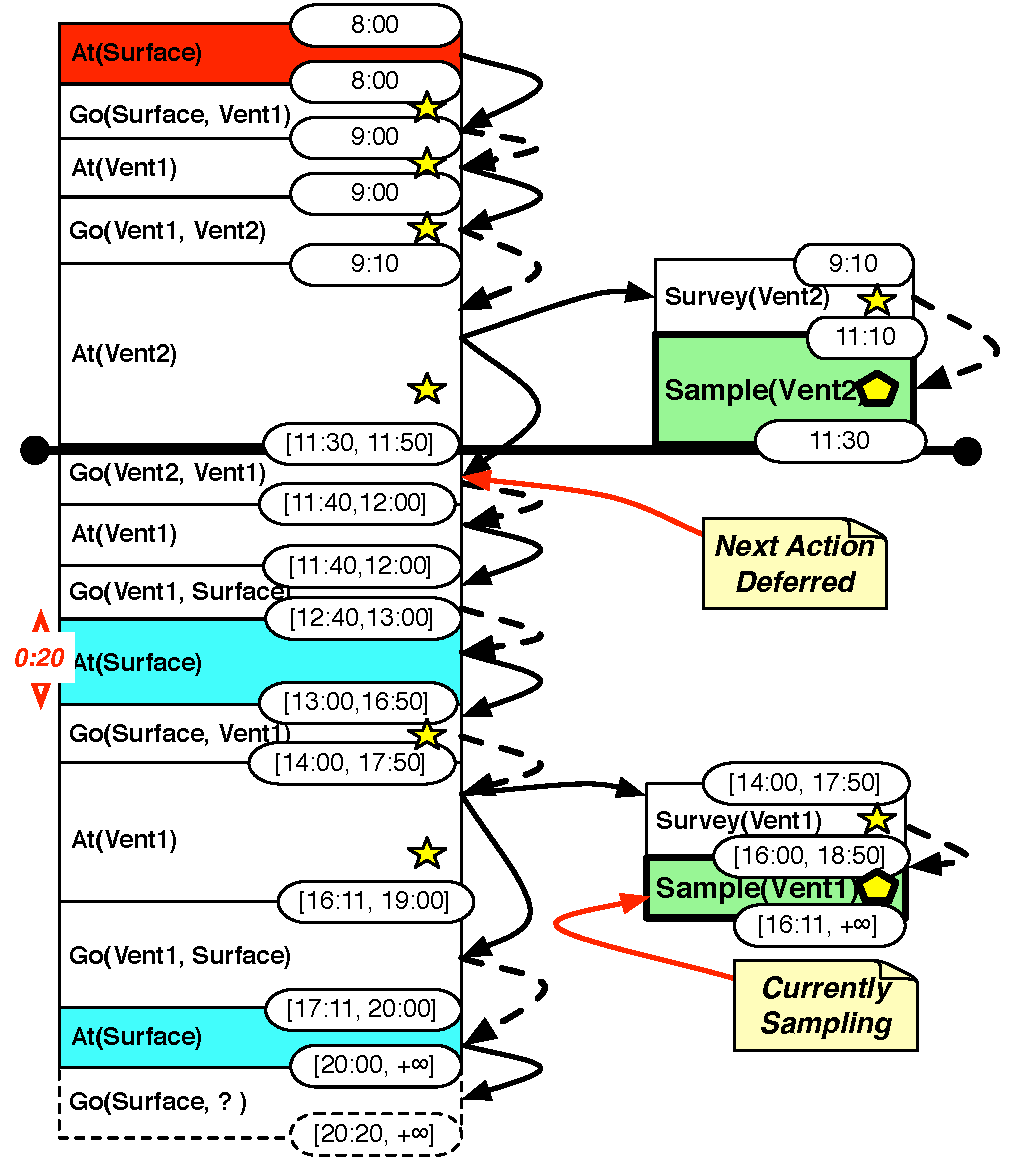
\includegraphics[width=0.7\columnwidth]{figs/example_ideal}
  \caption{\small The ideal plan solution for Fig. \ref{fig:ex:mixed2}. The
  thick line at 11:30 indicates the current time. Since {\em At Surface} is
  constrained to be at 13:00, the AUV would be stuck for 30 minutes which is
  not an efficient use of time.}
  \label{fig:res:ideal}
  \vskip-7mm
\end{figure}
 
Such refinement can be done only by considering the temporal
% constraints applied to plan timepoints. Should the {\em Surface} not
% have been constrained to be around 13:00 pm starting its execution
% proactively would have not blocked the vehicle at the surface. We
% plan, in the future, to explore how both the marking of the goals {\em
%   as urgent} and propagation to action can be better deduced by
% analyzing the simple temporal network (STN) supporting the current
% plan. Further, as the planner we used did not implement STNU and the
% work presented in \cite{morris01} about dynamic controllability. We
% believe that as this work is handled during planning while our
% approach is handled during plan execution, both should be easily
% complementary still the {\bf wait} actions inserted by their algorithm
% may need to be considered with a non urgent status within our
% approach.
constraints applied to the plan timepoints. Should the
{\em Surface} not have been constrained to be around 13:00 starting
its execution proactively would not have blocked the vehicle at the
surface. We hope to explore how both the marking of the goals {\em as
  urgent} and propagation to action can be better deduced by analyzing
the STN supporting the current plan. The insertion of {\bf wait}
actions during planning in \cite{morris01} and the possibility of
using STNUs within our plan representation, also needs investigation
with extensions to execution time changes in plan structure.

% Further, the planner we used did
% not implement STNU or the work presented in \cite{morris01} about
% dynamic controllability. We believe that as this work is handled
% during planning while our approach is handled during plan execution
% both should be easily complementary. Still the {\bf wait} actions
% inserted by their algorithm may need to be considered with a non
% urgent status within our approach.

Such refinements are likely to improve overall execution in our agent
despite uncertainty in the number and nature of goals during mission
execution. 
% All of these refinements are considered in order to further improve
% our approach in the context of temporal planning. They would allow
% further improvement in the overall execution of our agent despite the fact
% that the set of goals it will receive is not fully known until mission 
% completion.
In our domain such a requirement is critical as our AUV is in a
dynamic environment and it is far more cost-effective to use the
limited resources (scientists and on-station time) judiciously.  The
traditional approach to such AUV surveys has been to separate
exploration and exploitation into two different surveys
\cite{Yoerger01012007}.  By improving how the vehicle handles the
inclusion of new goals, we can greatly improve the efficacy of such
surveys while generalizing to other domains.





% While there has already been work around the topic of robust
% \fcomment{This is just a quick presentation on potential future
%   direction} As we stated in the related works our approach does not
% really address dynamic controllability and has the more classic
% assumption present in many planning frameworks that time-points are
% controllable. A side effect of this is that in its current state it
% may result on the system to decide to defer action as late as
% possible. In our example, this would result on the AUV leaving Vent1
% as late as 19:00 making the rest of its plan brittle to any delay due
% for example to downward water currents on its way to the surface. This
% needs to be further addressed in the future and, especially, how our
% work can be integrated with work presented in \cite{morris01}.

% Further as of today, we consider that the qualification of the goal is
% predefined when the goal is submitted by the planner. It is possible
% though that part of this can be refined on some cases based on the
% nature of the goal. Looking back at our domain, one can note that the
% 2 goals provided are constrained differently on their start time;
% while {\em Sample Vent2} start time is limited only on its upper
% bound, the returning to surface conversely is constrained only on the
% lower bound of its start time. This difference hints on some of the
% issues we presented. While we do consider that explicit information of
% these goals help the plan execution to be improved when such
% information is not initially present. We also are aware that the
% nature of the constraints within the goal itself can help identify the
% best policy to be done. It is obvious that for Sampling Vent2 it is
% better to be proactive on the actions that contribute to this
% goal. Conversely, the other goal only matter if it appears fairly late
% in the plan which means that it is probably better to not start
% completing this part of the plan too aggressively. We plan to further
% explore how we can refine the distinction between the different
% policies by using the information provided by the constraints of the
% different objectives.
 
%%% Local Variables: 
%%% mode: latex
%%% TeX-master: "aaai13"
%%% End: 


\twocolumn 
\bibliographystyle{aaai}
\bibliography{references}

\end{document}
